\documentclass[12pt,a4paper]{article}

% ── Packages ──────────────────────────────────────────────────────────────────
\usepackage[T1]{fontenc}
\usepackage[utf8]{inputenc}
\usepackage[margin=2.5cm]{geometry}
\usepackage{lmodern}
\usepackage{microtype}
\usepackage{xcolor}
\usepackage{graphicx}
\usepackage{float}
\usepackage{caption}
\usepackage{subcaption}
\usepackage{booktabs}
\usepackage{array}
\usepackage{tabularx}
\usepackage{multirow}
\usepackage{amsmath}
\usepackage{amssymb}
\usepackage{listings}
\usepackage{tikz}
\usetikzlibrary{shapes.geometric, arrows.meta, positioning, fit, backgrounds, calc}
\usepackage{pgfplots}
\pgfplotsset{compat=1.18}
\usepackage{tcolorbox}
\tcbuselibrary{skins, breakable}
\usepackage{enumitem}
\usepackage{titlesec}
\usepackage{fancyhdr}
\setlength{\headheight}{15pt}
\usepackage{hyperref}
\usepackage{parskip}
\usepackage{mdframed}
\usepackage{pifont}

% ── Colours ───────────────────────────────────────────────────────────────────
\definecolor{umons-blue}{HTML}{003366}
\definecolor{asp-green}{HTML}{27AE60}
\definecolor{t-blue}{HTML}{3498DB}
\definecolor{l-red}{HTML}{E74C3C}
\definecolor{plus-purple}{HTML}{9B59B6}
\definecolor{code-bg}{HTML}{F4F6F9}
\definecolor{code-border}{HTML}{BDC3C7}
\definecolor{verify-green}{HTML}{1E8449}

% ── Section style ─────────────────────────────────────────────────────────────
\titleformat{\section}{\Large\bfseries\color{umons-blue}}{{\thesection.}}{0.5em}{}[{\color{umons-blue}\titlerule[1.2pt]}]
\titleformat{\subsection}{\large\bfseries\color{umons-blue!80}}{\thesubsection.}{0.5em}{}
\titleformat{\subsubsection}{\normalsize\bfseries\color{umons-blue!60}}{\thesubsubsection.}{0.5em}{}
\titlespacing{\section}{0pt}{14pt}{6pt}
\titlespacing{\subsection}{0pt}{10pt}{4pt}

% ── Header / Footer ───────────────────────────────────────────────────────────
\pagestyle{fancy}
\fancyhf{}
\fancyhead[L]{\small\color{gray}KRR 2026 --- Non-Rectangular Tetracube Puzzles}
\fancyhead[R]{\small\color{gray}Agourzam \& El ismaily}
\fancyfoot[C]{\small\thepage}
\renewcommand{\headrulewidth}{0.4pt}

% ── ASP inline style ──────────────────────────────────────────────────────────
\lstdefinelanguage{ASP}{
  keywords={not,true,false},
  keywordstyle=\color{umons-blue}\bfseries,
  morecomment=[l]{\%},
  commentstyle=\color{gray}\itshape,
  sensitive=true
}
\lstset{basicstyle=\small\ttfamily, language=ASP,
        backgroundcolor=\color{code-bg},
        frame=single, rulecolor=\color{code-border},
        framesep=4pt, xleftmargin=6pt, xrightmargin=6pt,
        breaklines=true, keepspaces=true}

% ── Boxes ────────────────────────────────────────────────────────────────────
\newmdenv[backgroundcolor=t-blue!8,linecolor=t-blue,linewidth=1.2pt,
          innerleftmargin=12pt,innerrightmargin=12pt,
          innertopmargin=10pt,innerbottommargin=10pt,
          skipabove=10pt,skipbelow=10pt]{abstractbox}

\newmdenv[backgroundcolor=asp-green!8,linecolor=asp-green,linewidth=1.2pt,
          innerleftmargin=12pt,innerrightmargin=12pt,
          innertopmargin=8pt,innerbottommargin=8pt,
          skipabove=6pt,skipbelow=6pt]{contribbox}

% ── Checkmark / Crossmark ─────────────────────────────────────────────────────
\newcommand{\cmark}{\textcolor{verify-green}{\ding{51}}}
\newcommand{\xmark}{\textcolor{l-red}{\ding{55}}}

% ─────────────────────────────────────────────────────────────────────────────
\begin{document}

% ══════════════════════════════════════════════════════════════════════════════
% TITLE PAGE
% ══════════════════════════════════════════════════════════════════════════════
\begin{titlepage}
  \begin{tikzpicture}[remember picture, overlay]
    \fill[umons-blue] (current page.north west) rectangle
          ([yshift=-5cm]current page.north east);
    \fill[t-blue!70] ([yshift=-5cm]current page.north west) rectangle
          ([yshift=-5.5cm]current page.north east);
    \node[anchor=west, text=white, font=\Large\bfseries]
          at ([xshift=2.5cm, yshift=-2.2cm]current page.north west)
          {Final Report};
    \node[anchor=west, text=white!80, font=\normalsize]
          at ([xshift=2.5cm, yshift=-3.0cm]current page.north west)
          {Knowledge Representation and Reasoning, 2026};
    \node[anchor=west, text=white!60, font=\small]
          at ([xshift=2.5cm, yshift=-3.8cm]current page.north west)
          {Université de Mons (UMONS) --- Faculté des Sciences};
  \end{tikzpicture}

  \vspace*{5.8cm}

  {\LARGE\bfseries\color{umons-blue}
    Generating and Solving 3D Tetracube Puzzles\\[0.3cm]
    in Arbitrary Non-Rectangular Volumes with ASP}

  \vspace{0.5cm}
  \textcolor{umons-blue!60}{\rule{\linewidth}{1.5pt}}
  \vspace{0.5cm}

  \begin{tabular}{@{}ll}
    \textbf{Authors:}     & Abdelhadi Agourzam \quad|\quad Mohamed El ismaily \\[4pt]
    \textbf{Institution:} & Université de Mons (UMONS), Faculté des Sciences \\[4pt]
    \textbf{Supervisor:}  & Jef Wijsen \\[4pt]
    \textbf{Course:}      & Knowledge Representation and Reasoning, 2026 \\[4pt]
    \textbf{Date:}        & April 2026 \\[4pt]
    \textbf{Code:}        & \url{https://github.com/oscarRickovic/KRR2026}
  \end{tabular}

  \vspace{0.6cm}
  \textcolor{umons-blue!60}{\rule{\linewidth}{1pt}}
  \vspace{0.8cm}

  \begin{abstractbox}
    \textbf{Abstract.}
    We design and implement a \emph{shape-agnostic, scalable} system for
    generating and solving 3D tetracube puzzles using Answer Set Programming
    (ASP).  The 8 standard tetracubes (I, T, L, Pyramid, O, N, Z, Z-mirror)
    are packed into \emph{any} connected 3D volume by simply declaring its
    cells --- no shape-specific solver code is needed.  A single integer
    constant \texttt{num\_copies}\,$=N$ scales the puzzle to $8N$ pieces
    filling $32N$ cells, from the classical 32-cell problem ($N=1$) up to
    a 224-cell configuration ($N=7$).  We demonstrate solutions for three
    non-rectangular shapes (T-shape, L-shape, Plus/Cross) and randomly
    generated polycubes at multiple scales, with empirical solve times
    ranging from 30\,ms ($N=1$) to 6\,s ($N=7$).  An interactive 3D
    visualiser, an independent 6-check verifier, and a random puzzle
    generator complete the system.  All source code is available on GitHub.

    \vspace{4pt}
    \textbf{Keywords:} Answer Set Programming, Tetracubes, 3D Puzzle,
    Non-Rectangular Volumes, Shape-Agnostic, Scalable, Clingo, Exact Cover.
  \end{abstractbox}

  \vfill
  {\small\color{gray} University of Mons (UMONS) --- 2026}
\end{titlepage}

\tableofcontents
\clearpage

% ══════════════════════════════════════════════════════════════════════════════
\section{Introduction}
% ══════════════════════════════════════════════════════════════════════════════

A \textbf{tetracube} is a three-dimensional solid composed of four unit cubes
joined face-to-face.  There are exactly 8 distinct one-sided tetracube types.
Together they cover $8 \times 4 = 32$ unit cubes, suggesting the classical
puzzle: \emph{can all 8 pieces be packed into a given 3D volume with no gaps
and no overlaps?}

Existing work focuses on rectangular prisms ($2\times4\times4$,
$2\times2\times8$, etc.).  This project asks a more general question:

\begin{center}
\emph{Can the same ASP engine solve the puzzle for \textbf{any} connected
3D volume, and for \textbf{any number of copies} of the 8 pieces?}
\end{center}

The answer is yes --- in the sense that one unmodified engine \emph{accepts}
any such volume as input and returns a correct verdict (a packing, or a proof
that none exists).  This is a statement about the generality of the engine, not
a claim that every volume is packable: as Section~7 shows, most freely-shaped
3D volumes admit no packing at all.  The generality rests on two design choices:
\begin{enumerate}[leftmargin=1.8em]
  \item \textbf{Shape abstraction.}  The target volume is described entirely
        by a set of \texttt{cell(X,Y,Z)} facts.  The puzzle engine never
        references specific coordinates --- it only enforces boundary, non-overlap,
        and full coverage relative to whichever cells are declared.
  \item \textbf{Copy scaling.}  A single constant \texttt{num\_copies}\,$=N$
        multiplies the piece count to $8N$ and the required cell count to $32N$.
        Shapes accommodate this by extending their depth to $2N$ layers.
\end{enumerate}

\subsection{Contributions}

\begin{contribbox}
\begin{enumerate}[leftmargin=1.5em, label=\textbf{C\arabic*.}]
  \item \textbf{Shape-agnostic ASP engine.}  Three non-rectangular
        configurations (T, L, Plus/Cross) and arbitrary random polycubes
        are all solved by the same unmodified \texttt{puzzle.lp}.
  \item \textbf{Scalable num\_copies architecture.}  Changing $N$ from 1 to 7
        scales the problem from 32 to 224 cells without touching any solver code.
  \item \textbf{Automated rotation generation.}  All 86 distinct tetracube
        orientations are derived programmatically from 24 rotation matrices.
  \item \textbf{Configurable puzzle generation.}  A hint system with random
        seed produces puzzle instances at six difficulty levels for any $N$.
  \item \textbf{Independent verification.}  A 6-check Python verifier
        confirms solution correctness without trusting the solver output.
  \item \textbf{Interactive 3D visualiser.}  A matplotlib viewer with
        Puzzle/Solution toggle adapts automatically to any $N$.
  \item \textbf{Empirical complexity study.}  Solve times measured for
        $N=1$ to $N=7$ reveal a polynomial growth law $\sim N^{2.5}$.
\end{enumerate}
\end{contribbox}

% ══════════════════════════════════════════════════════════════════════════════
\section{The Eight Tetracube Pieces}
% ══════════════════════════════════════════════════════════════════════════════

Figure~\ref{fig:tetracubes3d} shows all 8 tetracubes in 3D.  Each piece is
a distinct connected solid of 4 unit cubes.  Their rotation counts (3 to 24)
reflect their symmetry: high-symmetry pieces (I, O) have few orientations;
the fully asymmetric L piece has 24.  The Pyramid is the only non-planar
piece --- it cannot be flattened into a single layer.

\begin{figure}[H]
  \centering
  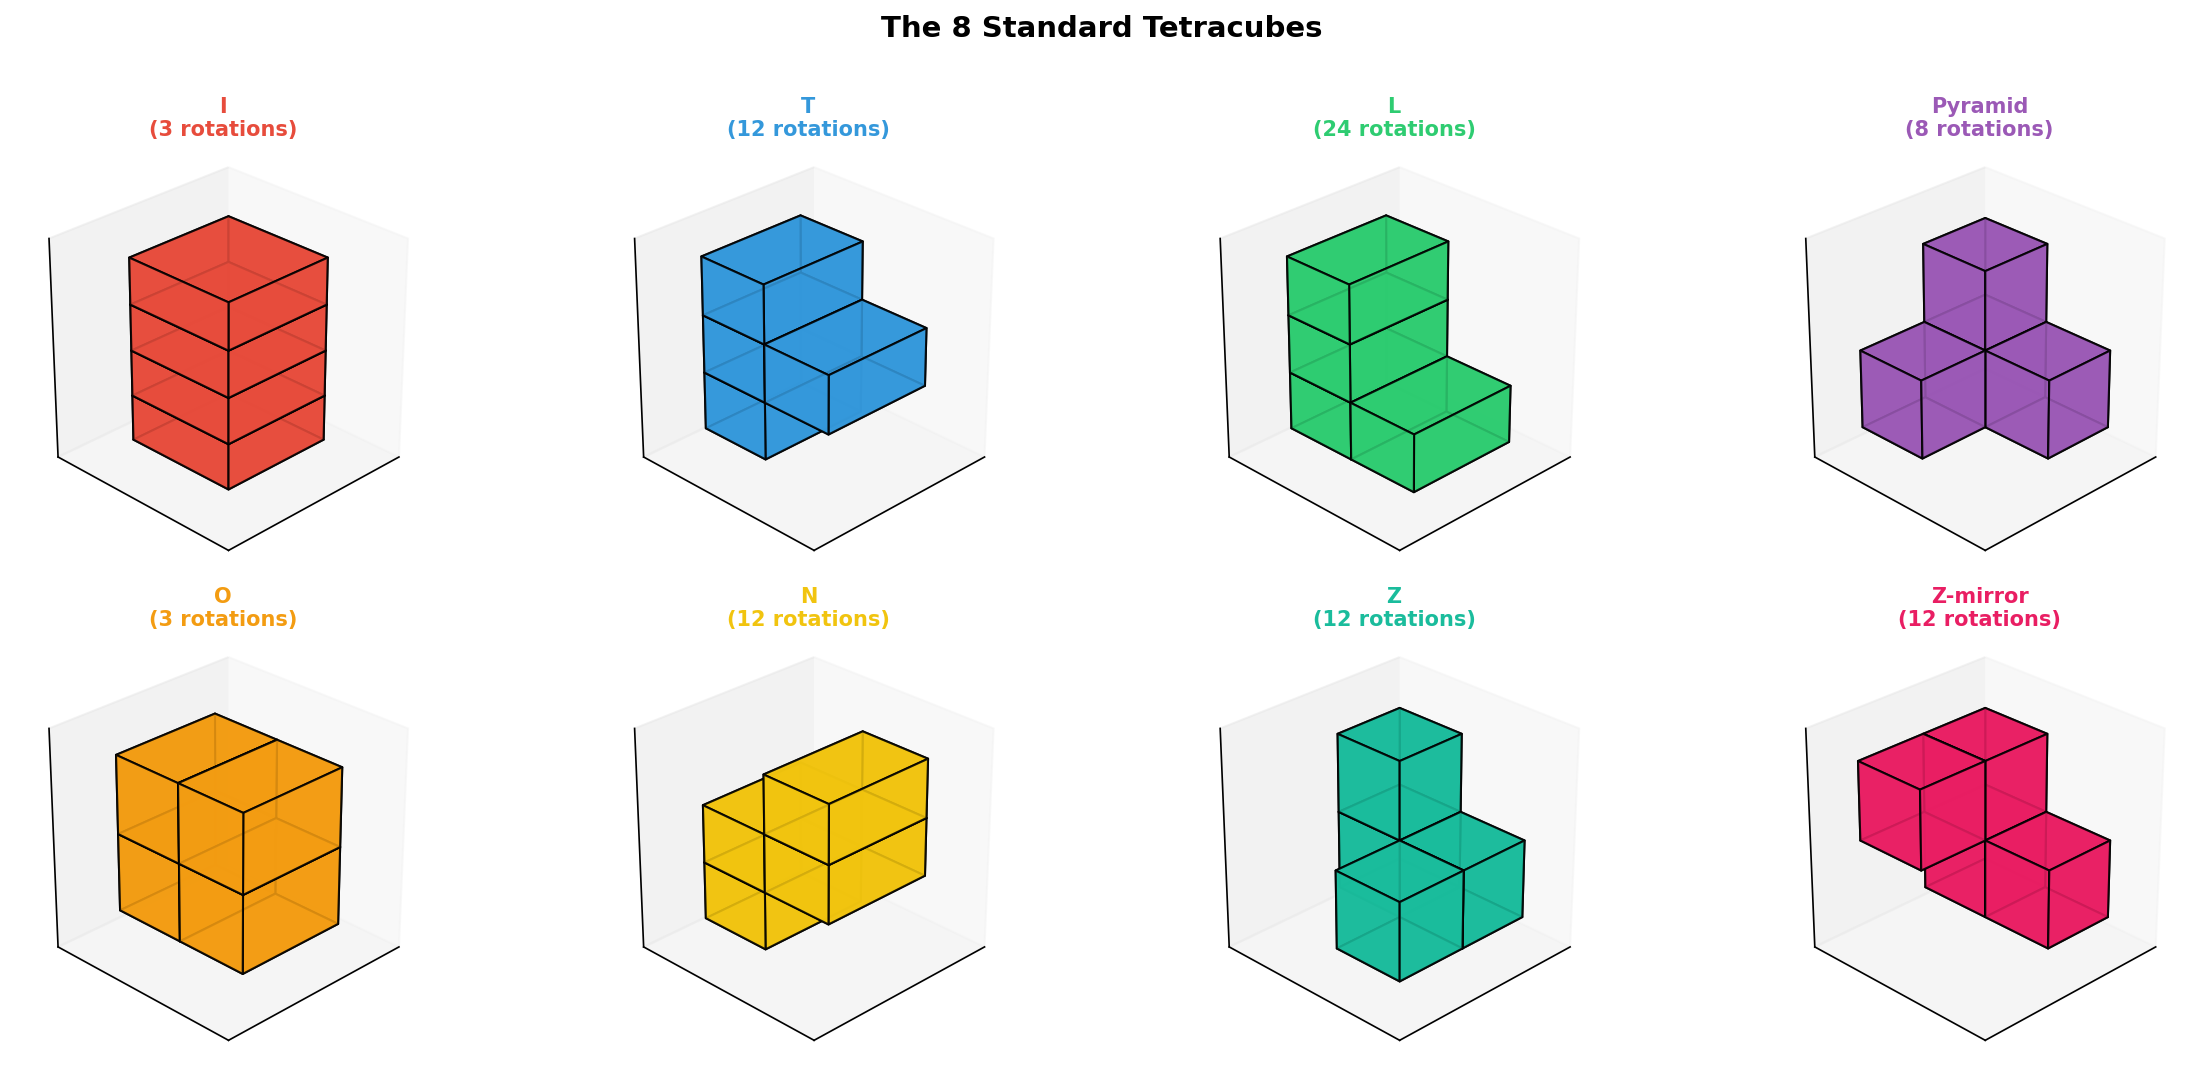
\includegraphics[width=\linewidth]{figures/fig_tetracubes_3d.png}
  \caption{All 8 standard tetracubes rendered in 3D, shown in their base
           orientation.  Each piece is coloured distinctly and labelled with
           its rotation count.  The Pyramid is the only piece that genuinely
           occupies three spatial dimensions.}
  \label{fig:tetracubes3d}
\end{figure}

\begin{table}[H]
\centering
\caption{Properties of the 8 standard tetracubes.}
\label{tab:pieces}
\renewcommand{\arraystretch}{1.3}
\begin{tabularx}{\linewidth}{@{}l c c X@{}}
  \toprule
  \textbf{Piece} & \textbf{Rotations} & \textbf{Type} & \textbf{Geometric property} \\
  \midrule
  I         &  3 & Planar        & Straight line along one axis; 3-fold axis symmetry. \\
  T         & 12 & Planar        & T-branch; central cube has one perpendicular neighbour. \\
  L         & 24 & Planar        & Hook; chiral and fully asymmetric, hence 24 orientations. \\
  Pyramid   &  8 & \textbf{3D}   & 3 cubes on base + 1 elevated; only genuinely 3D piece. \\
  O         &  3 & Planar        & $2\times2$ square slab; highest symmetry of all pieces. \\
  N         & 12 & Planar        & Zigzag; 2 offset rows of 2. \\
  Z         & 12 & Planar        & S-shape (right-handed); distinct from its mirror. \\
  Z-mirror  & 12 & Planar        & Mirror image of Z (left-handed). \\
  \midrule
  \textbf{Total} & \textbf{86} & 7P + 1 3D & $8 \times 4 = 32$ unit cubes. \\
  \bottomrule
\end{tabularx}
\end{table}

% ══════════════════════════════════════════════════════════════════════════════
\section{Volume Configurations}
% ══════════════════════════════════════════════════════════════════════════════

\subsection{Three Non-Rectangular Shapes}

We define three non-rectangular 3D volumes, each with a 16-cell XY footprint
extruded to depth 2 (32 cells at $N=1$).  Figure~\ref{fig:shapes_empty}
shows their 3D structure.

\begin{figure}[H]
  \centering
  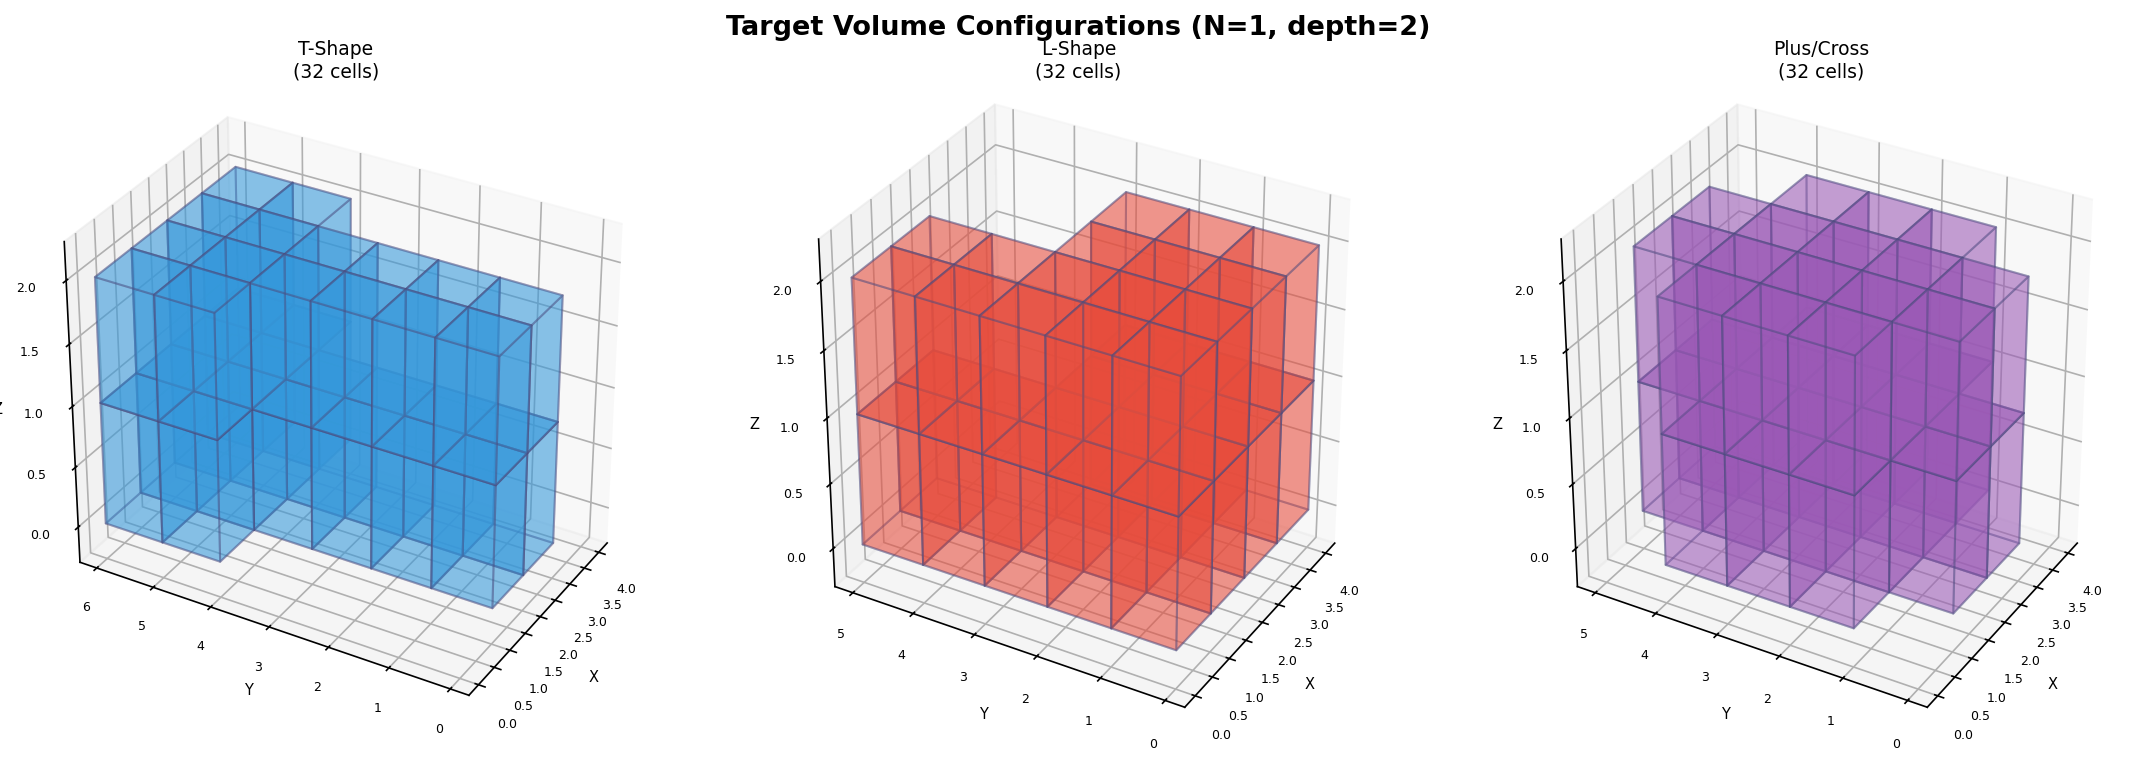
\includegraphics[width=\linewidth]{figures/fig_shapes_empty_3d.png}
  \caption{The three target volume configurations rendered in 3D (ghost view,
           $N=1$).  Left: T-Shape (bar + stem).  Centre: L-Shape
           (rectangle minus top-right corner).  Right: Plus/Cross
           (central body + top and bottom arms).  All contain exactly 32 cells.}
  \label{fig:shapes_empty}
\end{figure}

\textbf{T-Shape.}
A wide horizontal bar ($4\times2$ per layer) joined to a narrow stem
($2\times4$ per layer), with no overlap:
\[
  \text{T-shape} =
  \bigl(\{0..3\}\times\{4,5\}\bigr)
  \cup
  \bigl(\{1,2\}\times\{0..3\}\bigr)
  \times\{0,1\}
  \quad\longrightarrow\quad 32 \text{ cells}.
\]

\textbf{L-Shape.}
A $4\times5$ rectangle per layer with the top-right $2\times2$ corner
removed --- a staircase profile:
\[
  \text{L-layer} = [0..3]\times[0..4]
  \;\setminus\;
  \{x\geq2,\,y\geq3\}
  \quad\longrightarrow\quad 16 \text{ cells/layer}.
\]

\textbf{Plus/Cross.}
A symmetric plus shape: $4\times3$ central body plus $2\times1$ arms at top
and bottom:
\[
  \text{Plus-layer} =
  \{0..3\}\times\{1..3\}
  \;\cup\;
  \{1,2\}\times\{4\}
  \;\cup\;
  \{1,2\}\times\{0\}
  \quad\longrightarrow\quad 16 \text{ cells/layer}.
\]

\subsection{Scaling with \texttt{num\_copies}}

The \texttt{num\_copies}\,$=N$ parameter extends each shape's depth to $2N$
layers, giving exactly $32N$ cells for $8N$ pieces.  Geometrically, the XY
footprint is preserved while the Z-dimension doubles per copy.

\[
  N \text{ copies}
  \;\xrightarrow{\quad}\;
  \underbrace{8N}_{\text{pieces}}
  \;\times\; 4\text{ cells}
  = 32N \text{ unit cells}
  \;\xrightarrow{\quad}\;
  \text{depth } 2N \text{ layers}
\]

Figure~\ref{fig:scaling} compares the T-shape and L-shape at $N=1$ (depth 2)
and $N=2$ (depth 4), illustrating how the volume grows purely in the Z
direction.

\begin{figure}[H]
  \centering
  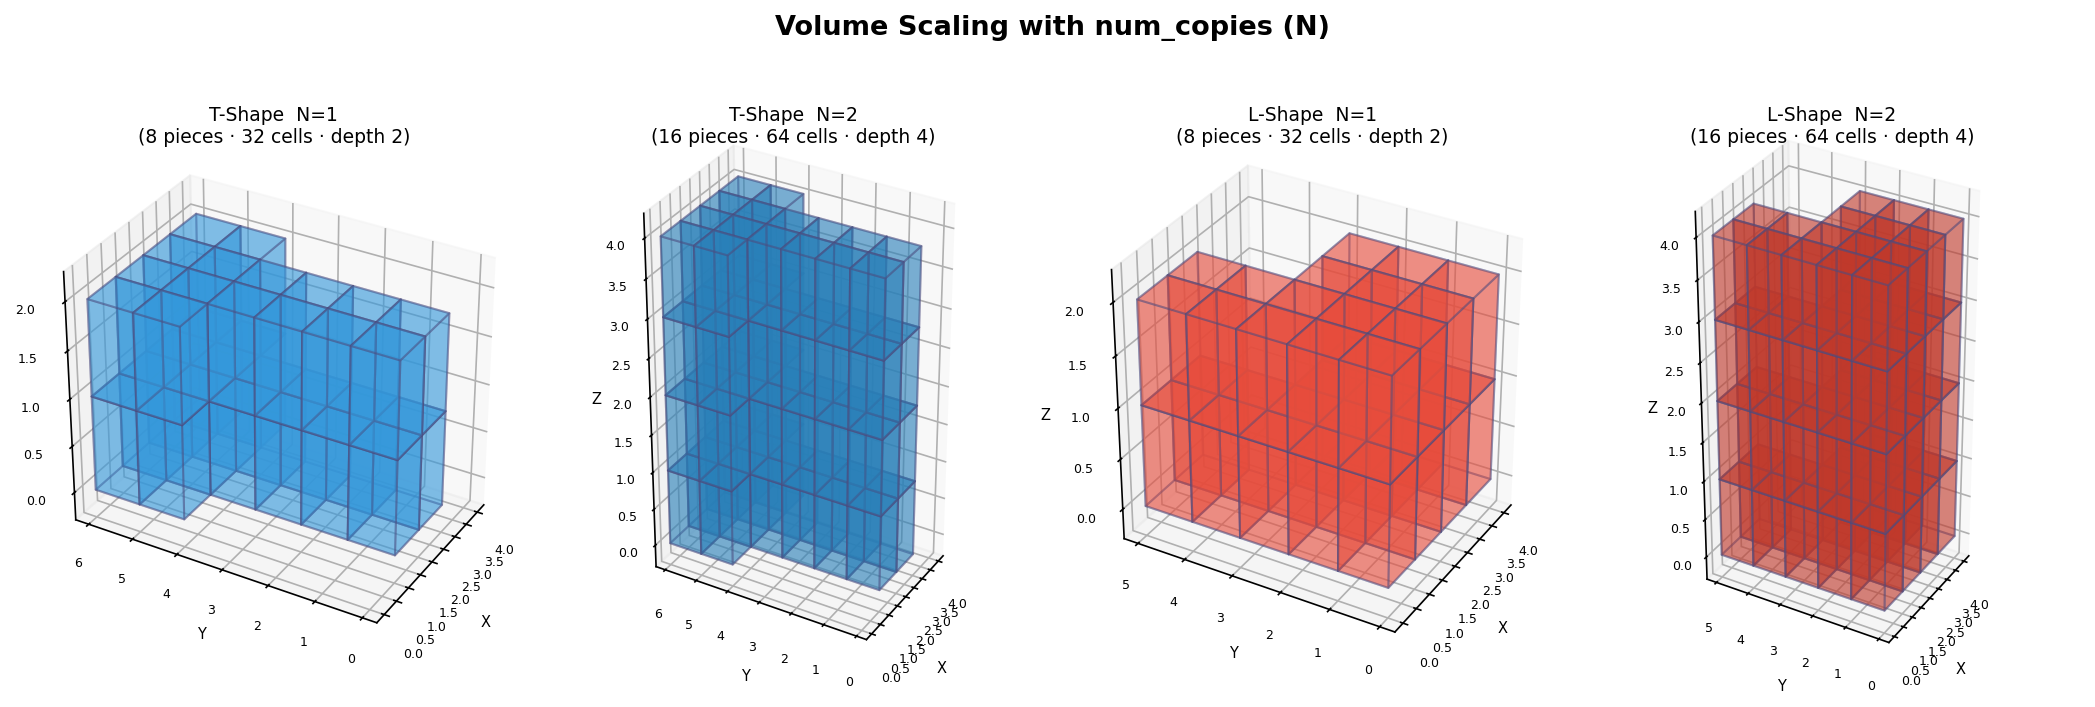
\includegraphics[width=\linewidth]{figures/fig_shape_scaling.png}
  \caption{Volume scaling with \texttt{num\_copies}.  The XY footprint is
           identical for $N=1$ (left) and $N=2$ (right); only the depth
           doubles.  T-Shape: 32 cells at $N=1$, 64 cells at $N=2$.
           L-Shape: same.  No shape-specific code changes.}
  \label{fig:scaling}
\end{figure}

\begin{table}[H]
\centering
\caption{Puzzle scale for \texttt{num\_copies} $N = 1$ to $7$.}
\label{tab:scale}
\renewcommand{\arraystretch}{1.2}
\begin{tabular}{@{}rrrrl@{}}
  \toprule
  $N$ & \textbf{Pieces} & \textbf{Cells} & \textbf{Depth ($z$)} & \textbf{Overlap pairs to check} \\
  \midrule
  1 &  8 &  32 & 0--1 &  28 \\
  2 & 16 &  64 & 0--3 & 120 \\
  3 & 24 &  96 & 0--5 & 276 \\
  4 & 32 & 128 & 0--7 & 496 \\
  5 & 40 & 160 & 0--9 & 780 \\
  6 & 48 & 192 & 0--11 & 1128 \\
  7 & 56 & 224 & 0--13 & 1540 \\
  \bottomrule
\end{tabular}
\end{table}

% ══════════════════════════════════════════════════════════════════════════════
\section{System Architecture}
% ══════════════════════════════════════════════════════════════════════════════

\subsection{Pipeline Overview}

The system consists of five components that interact in a linear pipeline.

\begin{figure}[H]
\centering
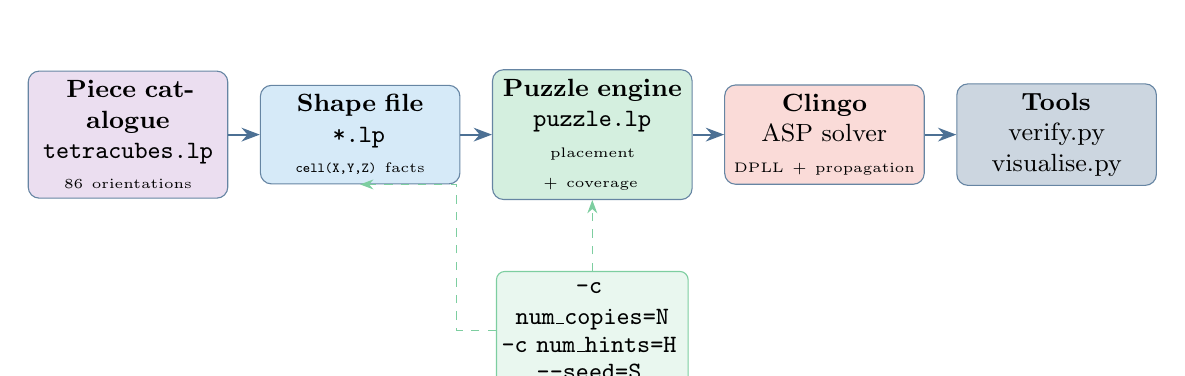
\begin{tikzpicture}[
  node distance=0.55cm and 0.4cm,
  box/.style={rectangle, rounded corners=4pt, draw=umons-blue!60,
              fill=umons-blue!10, minimum width=2.4cm, minimum height=1.1cm,
              text width=2.3cm, align=center, font=\small},
  param/.style={rectangle, rounded corners=3pt, draw=asp-green!60,
                fill=asp-green!10, minimum height=0.7cm,
                text width=2.2cm, align=center, font=\small},
  arr/.style={-Stealth, thick, umons-blue!70},
  parr/.style={-Stealth, dashed, asp-green!60}
]
  \node[box, fill=plus-purple!20] (pieces)
        {\textbf{Piece catalogue}\\{\small\texttt{tetracubes.lp}}\\{\tiny 86 orientations}};
  \node[box, fill=t-blue!20, right=of pieces] (shape)
        {\textbf{Shape file}\\{\small\texttt{*.lp}}\\{\tiny \texttt{cell(X,Y,Z)} facts}};
  \node[box, fill=asp-green!20, right=of shape] (puzzle)
        {\textbf{Puzzle engine}\\{\small\texttt{puzzle.lp}}\\{\tiny placement + coverage}};
  \node[box, fill=l-red!20, right=of puzzle] (clingo)
        {\textbf{Clingo}\\{\small ASP solver}\\{\tiny DPLL + propagation}};
  \node[box, fill=umons-blue!20, right=of clingo] (tools)
        {\textbf{Tools}\\{\small verify.py}\\{\small visualise.py}};

  \draw[arr] (pieces) -- (shape);
  \draw[arr] (shape)  -- (puzzle);
  \draw[arr] (puzzle) -- (clingo);
  \draw[arr] (clingo) -- (tools);

  % Parameters node below
  \node[param, below=0.9cm of puzzle] (param)
       {\texttt{-c num\_copies=N}\\[-1pt]\texttt{-c num\_hints=H}\\[-1pt]\texttt{--seed=S}};
  \draw[parr] (param.north) -- (puzzle.south);
  \draw[parr] (param.west) -- +(-0.5,0) |- (shape.south);

\end{tikzpicture}
\caption{End-to-end pipeline.  The shape file and \texttt{num\_copies} are the only
         inputs that change between configurations; all other components are reused.}
\label{fig:pipeline}
\end{figure}

\subsection{The \texttt{cell/3} Abstraction}

The core design insight is that the puzzle engine operates exclusively on the
\texttt{cell(X,Y,Z)} predicate, never on specific coordinates.  Adding a new
volume requires only a new file listing its cells.

The three fundamental constraints are:

\begin{enumerate}[leftmargin=1.8em, label=\textbf{(\arabic*)}]
  \item \textbf{Boundary.}  Every cube of every placed piece must land in a
        declared cell.
  \item \textbf{Non-overlap.}  No two distinct pieces may occupy the same cell.
  \item \textbf{Full coverage.}  Every declared cell must be occupied by exactly
        one piece.
\end{enumerate}

Together these three constraints constitute an \emph{exact cover} problem over
the cell set.  Clingo's DPLL-based propagation engine solves it efficiently.

\subsection{The \texttt{num\_copies} Scaling Mechanism}

The \texttt{num\_copies} parameter generalises the piece count without any
manual enumeration.  Piece IDs are assigned types through a cyclic formula:
piece $P$ receives the type at position $((P-1) \bmod 8) + 1$ in the
8-type sequence.  This ensures every copy of each type is represented exactly
once:

\begin{itemize}[leftmargin=1.8em]
  \item Pieces $1$--$8$ (copy 1): I, T, L, Pyramid, O, N, Z, Z-mirror
  \item Pieces $9$--$16$ (copy 2): same types, fresh IDs
  \item Pieces $8(k{-}1){+}1$ to $8k$ (copy $k$): same cycle
\end{itemize}

The shape files extend their Z-range to $0..2N{-}1$, providing exactly $32N$
cells.  The solver sees $8N$ pieces that must cover $32N$ cells exactly ---
the scale changes but the logical structure is identical at every $N$.

\subsection{Hint System and Puzzle Generation}

A \texttt{num\_hints} parameter selects a random subset of pieces to reveal
as ``given'' positions.  The remaining pieces become the puzzle to solve.
Six difficulty levels arise from varying the hint count from 7 (only 1 hidden
piece) to 0 (all $8N$ pieces hidden):

\begin{center}
\begin{tabular}{@{}lcc@{}}
  \toprule
  \textbf{Difficulty} & \textbf{Hints shown} & \textbf{Pieces to find ($N=1$)} \\
  \midrule
  Very Easy & 7   & 1 \\
  Easy      & 5--6 & 2--3 \\
  Medium    & 3--4 & 4--5 \\
  Hard      & 1--2 & 6--7 \\
  Harder    & 0   & 8 \\
  \bottomrule
\end{tabular}
\end{center}

\subsection{File Organisation}

\begin{table}[H]
\centering
\caption{Project files and their roles (full source on GitHub).}
\label{tab:files}
\renewcommand{\arraystretch}{1.25}
\begin{tabular}{@{}ll@{}}
  \toprule
  \textbf{File} & \textbf{Role} \\
  \midrule
  \texttt{tetracubes.lp}      & 86 rotation offsets for all 8 piece types \\
  \texttt{puzzle.lp}          & Shape-agnostic placement, coverage, hint logic; \texttt{num\_copies} \\
  \texttt{t\_shape.lp}        & T-shape cells ($32N$ total, depth $2N$) \\
  \texttt{l\_shape.lp}        & L-shape cells ($32N$ total, depth $2N$) \\
  \texttt{general\_shape.lp}  & Plus/Cross cells --- template for any shape \\
  \texttt{verify.py}          & Independent 6-check verifier; auto-detects $N$ \\
  \texttt{visualise.py}       & Interactive 3D viewer; auto-detects $N$ \\
  \texttt{random\_puzzle.py}  & Random shape generator with \texttt{--copies N} flag \\
  \texttt{benchmark.py}       & Timing comparison T vs L at multiple $N$ values \\
  \bottomrule
\end{tabular}
\end{table}

% ══════════════════════════════════════════════════════════════════════════════
\section{Solutions}
% ══════════════════════════════════════════════════════════════════════════════

The three non-rectangular volumes all admit valid tetracube packings,
confirmed by Clingo and independently verified.

\subsection{T-Shape Solution ($N=1$, 32 cells, 8 pieces)}

\begin{figure}[H]
  \centering
  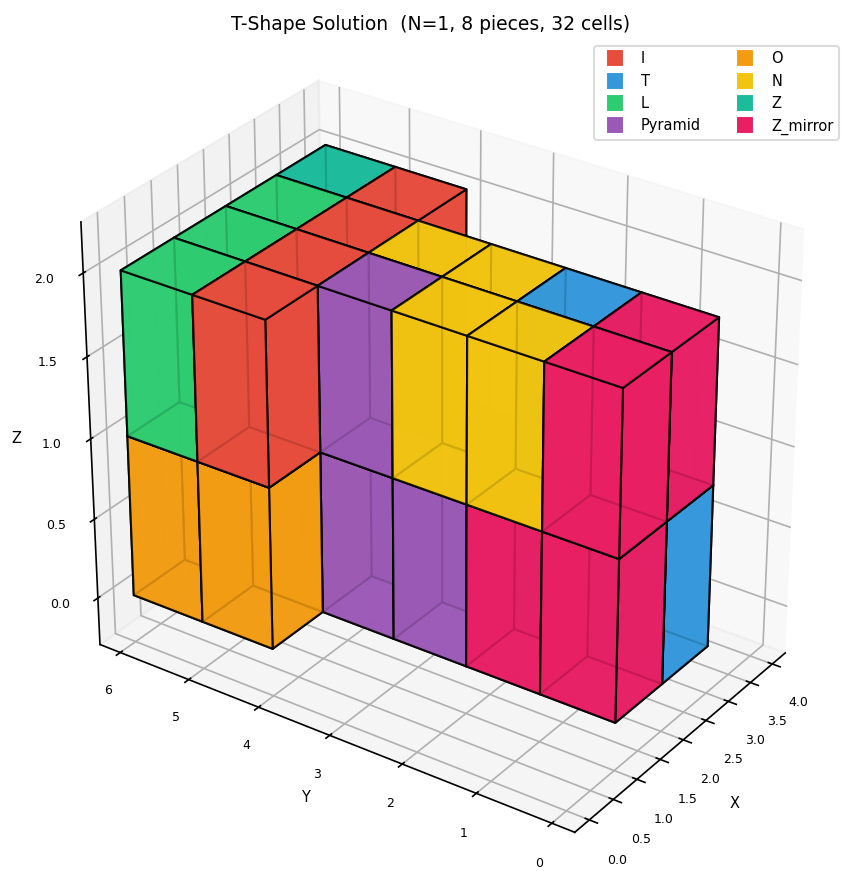
\includegraphics[width=0.75\linewidth]{figures/fig_solution_t.png}
  \caption{T-shape packed solution ($N=1$).  The semi-transparent ghost shows
           the volume boundary; each coloured solid is a distinct tetracube.
           Every cell is covered exactly once --- no gaps, no overlaps.}
  \label{fig:sol_t}
\end{figure}

\subsection{L-Shape Solution ($N=1$, 32 cells, 8 pieces)}

\begin{figure}[H]
  \centering
  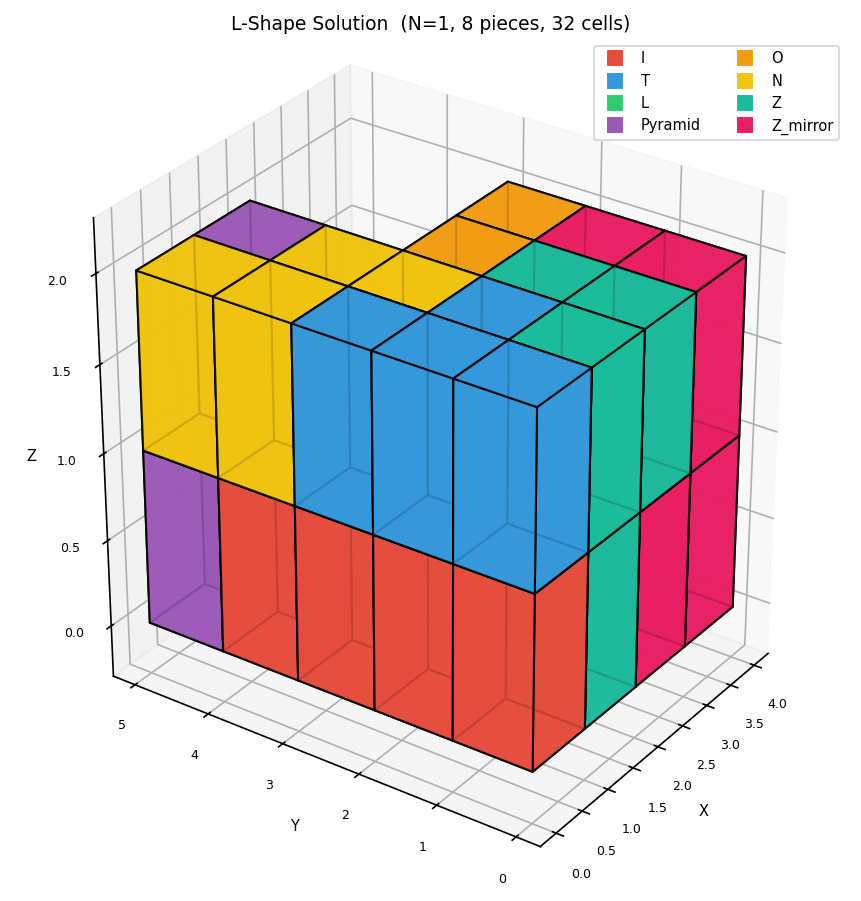
\includegraphics[width=0.75\linewidth]{figures/fig_solution_l.png}
  \caption{L-shape packed solution ($N=1$).  The staircase boundary is
           fully covered.  The asymmetric boundary forces different piece
           orientations than the T-shape, yet the same engine finds a valid
           packing.}
  \label{fig:sol_l}
\end{figure}

\subsection{Plus/Cross Solution ($N=1$, 32 cells, 8 pieces)}

\begin{figure}[H]
  \centering
  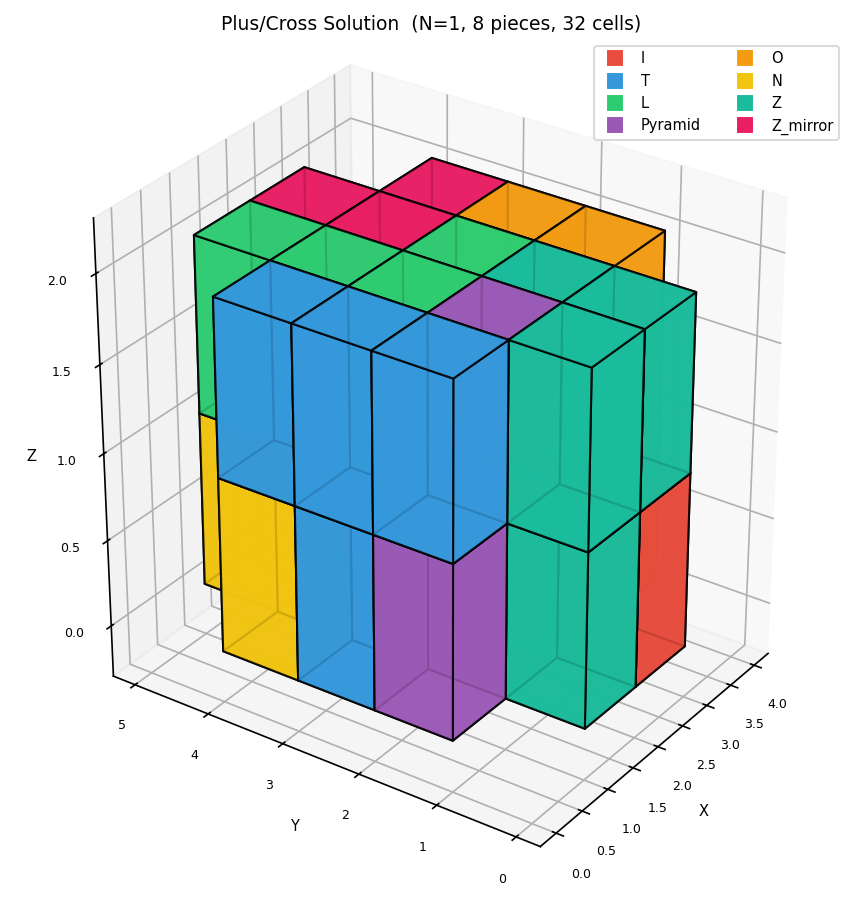
\includegraphics[width=0.75\linewidth]{figures/fig_solution_cross.png}
  \caption{Plus/Cross packed solution ($N=1$).  The non-convex boundary with
           four arms is entirely covered.  This is the most geometrically
           constrained of the three shapes --- the solver must fill the
           corner-less arms with appropriately oriented pieces.}
  \label{fig:sol_cross}
\end{figure}

\subsection{T-Shape Solution ($N=2$, 64 cells, 16 pieces)}

\begin{figure}[H]
  \centering
  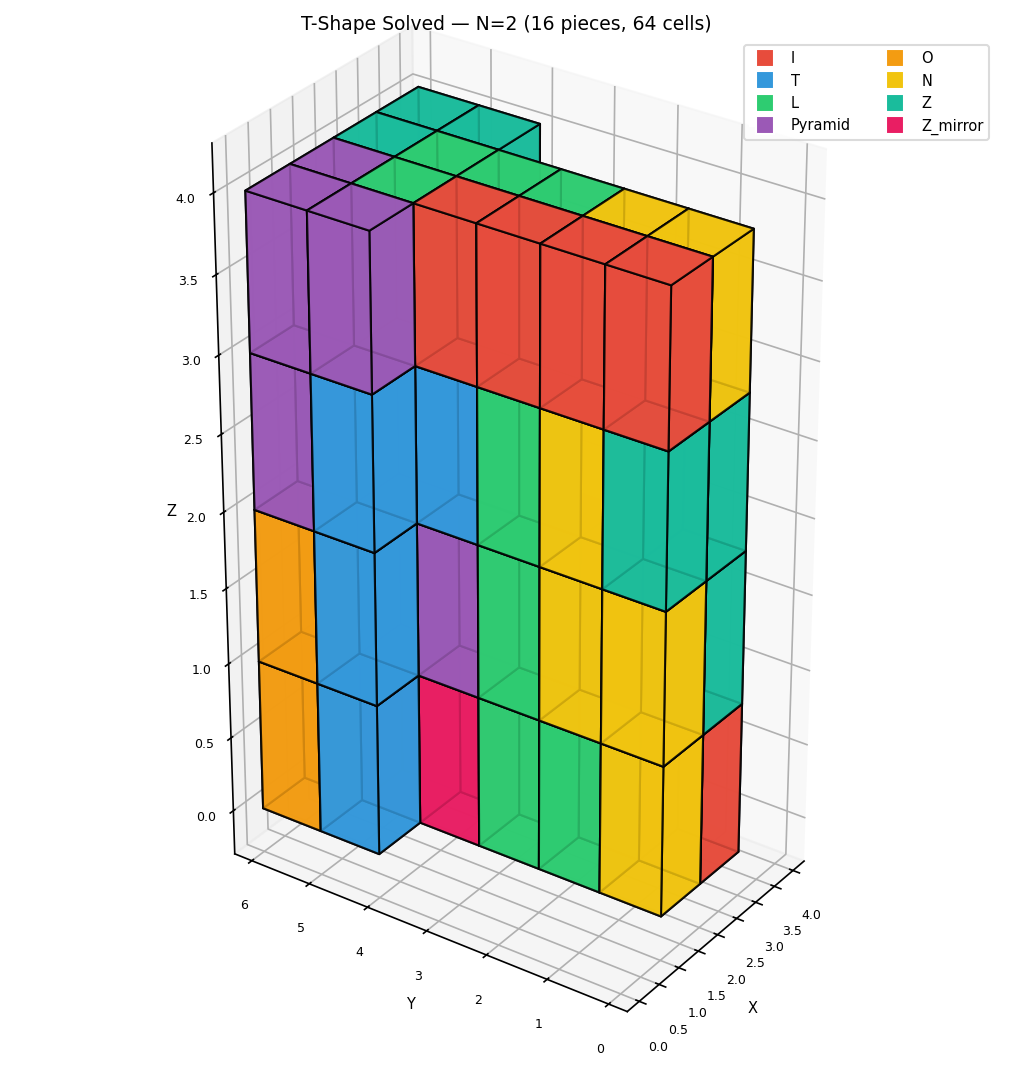
\includegraphics[width=0.75\linewidth]{figures/fig_solution_t2.png}
  \caption{T-shape packed solution ($N=2$): two stacked T-slabs forming a
           64-cell volume covered by 16 tetracubes.  The same solver algorithm
           scales from $N=1$ to $N=2$ with no code changes.}
  \label{fig:sol_t2}
\end{figure}

\subsection{Random Polycube Puzzles}

The \texttt{random\_puzzle.py} script demonstrates that the engine generalises
to \emph{any} connected 32-cell volume.  A random 16-cell polyomino is grown
using the Eden model (sequential random face-neighbour addition) and extruded
to depth 2.  Figure~\ref{fig:random} shows three solved random instances.

\begin{figure}[H]
  \centering
  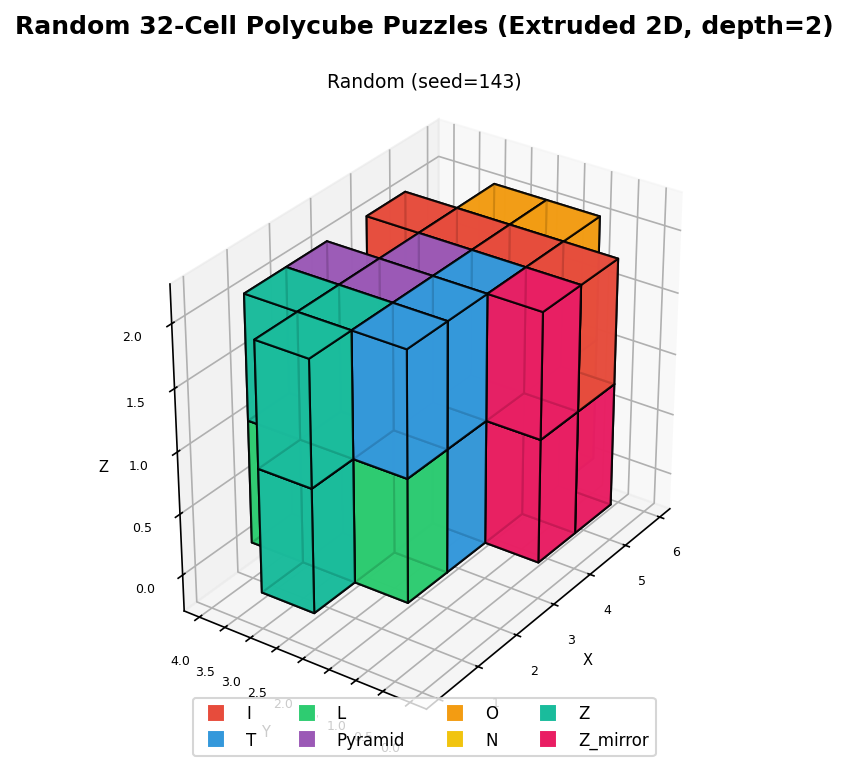
\includegraphics[width=\linewidth]{figures/fig_random_shapes.png}
  \caption{Three randomly generated 32-cell polycube puzzles and their
           solutions.  Each shape was grown by the Eden model with a different
           random seed.  Despite their irregular geometry, all three are solved
           by the same unmodified puzzle engine in under 50\,ms.}
  \label{fig:random}
\end{figure}

% ══════════════════════════════════════════════════════════════════════════════
\section{Independent Verification}
\label{sec:verify}
% ══════════════════════════════════════════════════════════════════════════════

An independent Python verifier (\texttt{verify.py}) re-derives the solution
from scratch and applies six checks without trusting Clingo.  The verifier
auto-detects $N$ from the \texttt{numCopies} atom in the answer set.

\begin{table}[H]
\centering
\caption{Verification results for T-shape and L-shape at $N = 1, 2, 3$.
         All configurations pass all six checks.}
\label{tab:verify}
\renewcommand{\arraystretch}{1.3}
\begin{tabular}{@{}clcccccc@{}}
  \toprule
  & & \multicolumn{2}{c}{$N=1$} & \multicolumn{2}{c}{$N=2$} & \multicolumn{2}{c}{$N=3$} \\
  \cmidrule(lr){3-4}\cmidrule(lr){5-6}\cmidrule(lr){7-8}
  & \textbf{Check} & T & L & T & L & T & L \\
  \midrule
  1 & Correct piece count \& type distribution & \cmark&\cmark&\cmark&\cmark&\cmark&\cmark \\
  2 & Rotation IDs within valid range per type  & \cmark&\cmark&\cmark&\cmark&\cmark&\cmark \\
  3 & All piece cells within declared cell set  & \cmark&\cmark&\cmark&\cmark&\cmark&\cmark \\
  4 & No two pieces share a cell               & \cmark&\cmark&\cmark&\cmark&\cmark&\cmark \\
  5 & All $32N$ cells covered                  & \cmark&\cmark&\cmark&\cmark&\cmark&\cmark \\
  6 & Hint IDs are a subset of placed IDs      & \cmark&\cmark&\cmark&\cmark&\cmark&\cmark \\
  \midrule
  \multicolumn{2}{@{}l}{\textbf{Verdict}} &
    \multicolumn{2}{c}{\textcolor{verify-green}{\textbf{PASS}}} &
    \multicolumn{2}{c}{\textcolor{verify-green}{\textbf{PASS}}} &
    \multicolumn{2}{c}{\textcolor{verify-green}{\textbf{PASS}}} \\
  \bottomrule
\end{tabular}
\end{table}

% ══════════════════════════════════════════════════════════════════════════════
\section{Complexity Analysis}
% ══════════════════════════════════════════════════════════════════════════════

\subsection{Problem Complexity}

\textbf{NP membership.}  Tetracube packing is in $\mathbf{NP}$: given a
placement for all $8N$ pieces, correctness can be verified in polynomial time
by checking boundary ($O(N)$), non-overlap ($O(N^2)$ pairs), and coverage
($O(N)$).  This is exactly what \texttt{verify.py} does.

\textbf{The decision problem.}  The ``answer is yes'' of Section~1 concerns the
\emph{generality of the engine}, not satisfiability.  The associated decision
problem is genuinely two-sided:

\begin{center}
\emph{given a connected polycube $V$ with $|V| = 32k$, can $V$ be partitioned
into exactly $k$ copies of each of the 8 tetracube types (rotations allowed)?}
\end{center}

This problem has both yes- and no-instances --- indeed, most freely-grown 3D
polycubes are no-instances (Section~7.4, Table~\ref{tab:bench3d}).  The T-, L-
and Plus volumes are \emph{not} hardness witnesses: they are satisfiable by
construction (Section~7.4) and merely demonstrate that the engine works.

\textbf{NP-hardness (conjectured).}  Packing a region with an \emph{arbitrary}
tile set is NP-complete~\cite{demaine2007,gareyjohnson1979}, and tiling with a
\emph{fixed} set of simple tiles is NP-complete as well~\cite{moore2001}.  This
strongly suggests our fixed-8-type problem is NP-hard, but a complete reduction
is left as future work.  We therefore make no worst-case running-time claim;
the timing of Section~7.3 measures one structured, easy family only.

\subsection{Configuration Space and Grounding Size}

The following counts the size of the naive configuration space (equivalently,
the number of ground placement atoms the solver must reason over).  We stress
that this is \emph{not} a bound on running time --- much as the $N!$ permutations
of a list do not imply that sorting takes factorial time.  It only indicates how
large the unpruned space is, motivating why structure and propagation matter.
A rough upper bound on placement choices is:
\[
  \text{Search space} \;\lesssim\;
  \underbrace{(32N \times 86)^{8N}}_{\text{position} \times \text{rotation for each piece}}
  \;\div\;
  \underbrace{(N!)^8}_{\text{interchangeable copies}}
\]

The denominator accounts for symmetry between the $N$ copies of each type.
In practice, Clingo's unit propagation eliminates the vast majority of this
space: placing one piece immediately constrains where others can go, often
reducing the effective branching factor to near 1 per decision.

\begin{table}[H]
\centering
\caption{ASP grounding size (approximate) as a function of $N$.}
\label{tab:ground}
\renewcommand{\arraystretch}{1.2}
\begin{tabular}{@{}rrrrrr@{}}
  \toprule
  $N$ & Cells & Pieces & Rotations & Anchor choices & Position atoms\\
  \midrule
  1 &  32 &  8 & 86 &   2\,752 &   22\,016 \\
  2 &  64 & 16 & 86 &   5\,504 &   88\,064 \\
  3 &  96 & 24 & 86 &   8\,256 & 198\,144 \\
  4 & 128 & 32 & 86 &  11\,008 & 352\,256 \\
  7 & 224 & 56 & 86 &  19\,264 & 1\,078\,784 \\
  \bottomrule
\end{tabular}
\end{table}

\subsection{Empirical Timing: $N = 1$ to $7$}

Table~\ref{tab:timing} and Figure~\ref{fig:perf} report measured Clingo
solve times for the T-shape and L-shape at all $N$ from 1 to 7, at maximum
difficulty (0 hints), averaged over 3 random seeds.

\begin{table}[H]
\centering
\caption{Average solve time (seconds) for T-shape and L-shape, $N=1$ to $N=7$.
         Difficulty: 0 hints (all pieces hidden). Averaged over seeds 43, 44, 45.}
\label{tab:timing}
\renewcommand{\arraystretch}{1.25}
\begin{tabular}{@{}rrrrrr@{}}
  \toprule
  $N$ & \textbf{Cells} & \textbf{Pieces} & \textbf{T-Shape (s)} & \textbf{L-Shape (s)} & \textbf{Slowdown (T)} \\
  \midrule
  1 &  32 &  8 & 0.030 & 0.030 & $1\times$ \\
  2 &  64 & 16 & 0.174 & 0.158 & $5.8\times$ \\
  3 &  96 & 24 & 0.441 & 0.413 & $14.7\times$ \\
  4 & 128 & 32 & 0.837 & 0.892 & $27.9\times$ \\
  5 & 160 & 40 & 1.673 & 1.855 & $55.8\times$ \\
  6 & 192 & 48 & 2.819 & 3.679 & $93.9\times$ \\
  7 & 224 & 56 & 3.986 & 6.012 & $132.9\times$ \\
  \bottomrule
\end{tabular}
\end{table}

\begin{figure}[H]
  \centering
  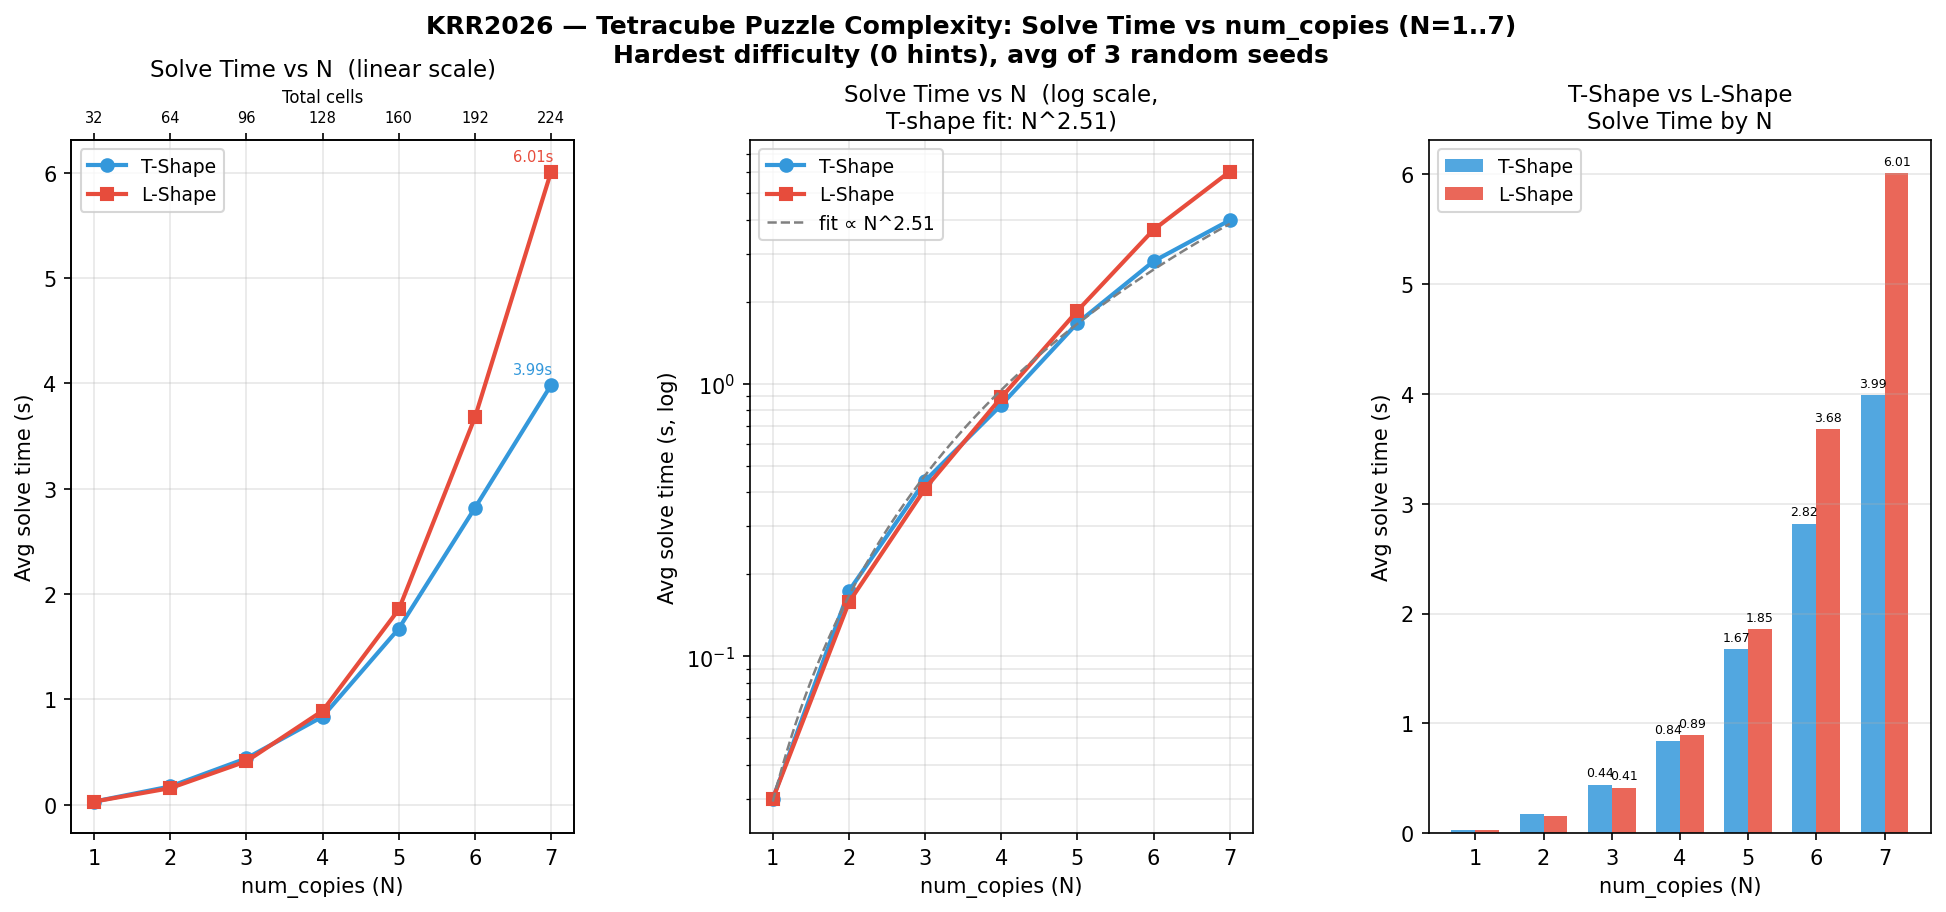
\includegraphics[width=\linewidth]{figures/fig_performance.png}
  \caption{Solve time vs \texttt{num\_copies} for T-shape (blue) and L-shape (red).
           \textbf{Left:} linear scale shows the absolute growth from 30\,ms
           to $\sim$6\,s over $N=1$--7.
           \textbf{Centre:} log scale reveals a power law; fitting gives
           $t \approx c \cdot N^{2.5}$ for the T-shape.
           \textbf{Right:} side-by-side bar chart comparing the two shapes at each $N$.}
  \label{fig:perf}
\end{figure}

\subsection{Scaling Analysis}

Several key observations emerge from the timing data:

\begin{enumerate}[leftmargin=1.8em]
  \item \textbf{The timed instances are easy by construction.}  Every shape
        here is a fixed 16-cell XY footprint extruded to depth $2N$ (a
        \emph{slab}).  Such instances are \emph{decomposable}: if the depth-2
        base ($N=1$) is packable, then the depth-$2N$ volume is packable by
        stacking $N$ vertically-translated copies of the base solution
        (copy $k$ occupying $z \in \{2k, 2k+1\}$; every tetracube, including
        the $2\times2\times2$ Pyramid, fits within two layers).  Hence
        satisfiability at $N=1$ \emph{implies} satisfiability at all $N$,
        constructively and in linear time.  The measured
        $t(N) \approx c \cdot N^{2.5}$ therefore characterises Clingo's
        behaviour on a structured, solution-dense family --- it is \emph{not}
        a worst-case bound for the general problem of Section~7.1.  (Clingo
        does not exploit the decomposition; it solves the monolithic exact
        cover, and the interchangeable copies even enlarge the grounding, so
        the polynomial growth reflects abundance of solutions plus strong
        propagation rather than intrinsic ease for the solver.)

  \item \textbf{Slab vs. general volumes.}  The slab construction is special
        precisely because it \emph{guarantees} a yes-instance.  Removing that
        structure changes the picture sharply: Table~\ref{tab:bench3d} shows
        that freely-grown 3D polycubes of the same sizes are almost never
        packable, and that even \emph{deciding} them becomes slower and more
        variable with $N$.  The slab timing should thus be read as a
        best-case, not a representative, scaling law.

  \item \textbf{L-shape harder than T-shape at large $N$.}  At $N=7$, the
        L-shape takes 6\,s vs 4\,s for the T-shape.  The L-shape's
        asymmetric boundary leaves fewer valid anchor positions for the
        longer pieces (I, N, Z), creating harder sub-problems.

  \item \textbf{Practical scalability.}  All instances up to $N=7$
        (224 cells, 56 pieces) solve in under 10 seconds.  This is
        well within interactive response time even at the largest tested scale.

  \item \textbf{Slowdown factor.}  From $N=1$ to $N=7$, T-shape slows by
        $133\times$.  With $N^{2.5}$ scaling this is consistent:
        $7^{2.5} / 1^{2.5} \approx 130$.
\end{enumerate}

\subsection{The General Case: Non-Decomposable 3D Volumes}

To probe the problem \emph{without} the slab guarantee, we generated free 3D
polycubes with the Eden model (\texttt{random\_puzzle.py --mode 3d}): each is a
connected $32N$-cell volume grown in all three axes, so its layers differ and no
stacking decomposition exists.  For each $N$ we generated shapes until 5
satisfiable instances were found or 400 attempts were exhausted, solving each at
maximum difficulty (0 hints) with a 30\,s timeout
(\texttt{benchmark\_3d.py}).

\begin{table}[H]
\centering
\caption{Free 3D polycubes (non-decomposable). Unlike the slab family, these
         are almost never packable, and the decision cost grows with $N$.}
\label{tab:bench3d}
\renewcommand{\arraystretch}{1.25}
\begin{tabular}{@{}rrrrrr@{}}
  \toprule
  $N$ & \textbf{Cells} & \textbf{Attempts} & \textbf{SAT rate} &
  \textbf{UNSAT mean (s)} & \textbf{Timeouts ($>30$\,s)} \\
  \midrule
  1 &  32 & 400 & $0.5\%$ & 0.028 & 0 \\
  2 &  64 & 400 & $0.0\%$ & 0.113 & 0 \\
  3 &  96 & 400 & $0.0\%$ & 0.399 & 1 \\
  \bottomrule
\end{tabular}
\end{table}

Two facts stand out.  First, satisfiability is \emph{rare}: out of 400 random
$64$- and $96$-cell polycubes, none admitted a packing, confirming that the
decision problem of Section~7.1 is genuinely two-sided and predominantly
negative.  Second, the cost of \emph{refuting} an instance grows with $N$
($0.028 \to 0.113 \to 0.399$\,s mean) and becomes variable --- one $N=3$
instance exceeded the 30\,s timeout.  This contrasts sharply with the smooth,
always-satisfiable slab curve of Section~7.3, and is the behaviour one expects
of a hard, two-sided problem rather than an easy structured one.

% ══════════════════════════════════════════════════════════════════════════════
\section{Conclusion}
% ══════════════════════════════════════════════════════════════════════════════

We have built a complete, shape-agnostic, scalable system for 3D tetracube
puzzles using Answer Set Programming.

\textbf{Key achievements:}
\begin{itemize}[leftmargin=1.8em]
  \item Three non-rectangular volumes (T, L, Plus/Cross) and arbitrary random
        polycubes are all solved by one unmodified solver algorithm.
  \item The \texttt{num\_copies} parameter scales the puzzle from 32 cells
        ($N=1$) to 224 cells ($N=7$) with no code changes.
  \item On the (decomposable) slab family, empirical timing from $N=1$ to
        $N=7$ grows polynomially, $t \approx c \cdot N^{2.5}$; this is a
        best-case scaling law, not a worst-case bound, since these instances
        are satisfiable by construction and stack from the $N=1$ solution.
  \item On free 3D polycubes the picture is the opposite: satisfiability is
        rare and decision cost grows with $N$, evidencing the genuinely
        two-sided, conjectured-NP-hard general problem.
  \item All slab solutions at $N=1$, $N=2$, $N=3$ pass 6 independent
        correctness checks.
\end{itemize}

\textbf{Design principle validated:}
Separating \emph{shape description} (\texttt{cell/3}) from \emph{puzzle logic}
(\texttt{puzzle.lp}), combined with the cyclic \texttt{num\_copies} scaling,
turns a shape-specific one-shot solver into a general puzzle framework.
This demonstrates ASP's strength: declarative constraints naturally
generalise over both geometry and scale.

\vspace{1cm}
\noindent\textcolor{umons-blue!60}{\rule{\linewidth}{1.5pt}}
\begin{center}
  \small\color{gray}
  Université de Mons (UMONS) --- Knowledge Representation and Reasoning, 2026\\
  Abdelhadi Agourzam \quad|\quad Mohamed El ismaily\\[2pt]
\end{center}

% ══════════════════════════════════════════════════════════════════════════════
\begin{thebibliography}{9}
\bibitem{demaine2007}
  E.~D. Demaine and M.~L. Demaine.
  \emph{Jigsaw Puzzles, Edge Matching, and Polyomino Packing: Connections and
  Complexity}.
  Graphs and Combinatorics, 23(Suppl 1):195--208, 2007.
\bibitem{moore2001}
  C.~Moore and J.~M. Robson.
  \emph{Hard Tiling Problems with Simple Tiles}.
  Discrete \& Computational Geometry, 26:573--590, 2001.
\bibitem{gareyjohnson1979}
  M.~R. Garey and D.~S. Johnson.
  \emph{Computers and Intractability: A Guide to the Theory of
  NP-Completeness}.
  W.~H. Freeman, 1979.
\end{thebibliography}

\end{document}
